% This file was converted to LaTeX by Writer2LaTeX ver. 1.4
% see http://writer2latex.sourceforge.net for more info
\documentclass[a4paper]{article}
\usepackage[ascii]{inputenc}
\usepackage[T1]{fontenc}
\usepackage[english]{babel}
\usepackage{amsmath}
\usepackage{amssymb,amsfonts,textcomp}
\usepackage{color}
\usepackage{array}
\usepackage{hhline}
\usepackage{hyperref}
\hypersetup{pdftex, colorlinks=true, linkcolor=blue, citecolor=blue, filecolor=blue, urlcolor=blue, pdftitle=, pdfauthor=, pdfsubject=, pdfkeywords=}
\usepackage[pdftex]{graphicx}
\newcommand\textsubscript[1]{\ensuremath{{}_{\text{#1}}}}
% Text styles
\newcommand\textstyleStrong[1]{\textmd{\MakeUppercase{#1}}}
\newcommand\textstyleEmphasis[1]{\textit{#1}}
\newcommand\textstyleInternetlink[1]{\textcolor[rgb]{0.0,0.0,0.5019608}{#1}}
\newcommand\textstylevmhook[1]{#1}
\newcommand\textstyletopichighlight[1]{#1}
\newcommand\textstyleStrongEmphasis[1]{\textbf{#1}}
\newcommand\textstyleFootnoteSymbol[1]{\textsuperscript{#1}}
% Outline numbering
\setcounter{secnumdepth}{0}
% Page layout (geometry)
\setlength\voffset{-1in}
\setlength\hoffset{-1in}
\setlength\topmargin{2cm}
\setlength\oddsidemargin{2cm}
\setlength\textheight{23.261cm}
\setlength\textwidth{17.001cm}
\setlength\footskip{0.0cm}
\setlength\headheight{1.27cm}
\setlength\headsep{1.169cm}
% Footnote rule
\setlength{\skip\footins}{0.119cm}
\renewcommand\footnoterule{\vspace*{-0.018cm}\setlength\leftskip{0pt}\setlength\rightskip{0pt plus 1fil}\noindent\textcolor{black}{\rule{0.25\columnwidth}{0.018cm}}\vspace*{0.101cm}}
% Pages styles
\makeatletter
\newcommand\ps@Standard{
  \renewcommand\@oddhead{}
  \renewcommand\@evenhead{}
  \renewcommand\@oddfoot{}
  \renewcommand\@evenfoot{}
  \renewcommand\thepage{\arabic{page}}
}
\newcommand\ps@FirstPage{
  \renewcommand\@oddhead{\textstyleStrong{\ IIT ROORKEE 2019-20}}
  \renewcommand\@evenhead{\@oddhead}
  \renewcommand\@oddfoot{}
  \renewcommand\@evenfoot{}
  \renewcommand\thepage{\arabic{page}}
}
\makeatother
\pagestyle{Standard}
\title{}
\author{}
\date{2019-11-01}
\begin{document}
\clearpage\setcounter{page}{1}\pagestyle{Standard}
\thispagestyle{FirstPage}
{\centering
CLUSTER COMPUTING\newline
CSN 221
\par}


\bigskip


\bigskip


\bigskip

{\centering
Leshna Balara \ \ \ \ \ \ \ \ \ \ 18114044
\par}

{\centering
Radhika \ \ \ \ \ \ \ \ \ \ \ \ \ \ \ \ \ \ \ \ 18114060
\par}

{\centering
Balne Niteesha \ \ \ \ \ \ \ \ \ \ 18114017 
\par}

{\centering
Karanpreet Singh \ \ \ \ \ 18114036
\par}

{\centering
Akshat Jain \ \ \ \ \ \ \ \ \ \ \ \ \ \ 18116006
\par}

{\centering
Armaan Pareek \ \ \ \ \ \ \ \ \ 18116017 
\par}

{\centering
Ashutosh Bharambe 18116019
\par}


\bigskip


\bigskip


\bigskip


\bigskip


\bigskip


\bigskip


\bigskip


\bigskip

{\centering
Submitted to: Assoc. Prof .Sateesh Kumar Peddoju
\par}


\bigskip

\section{Abstract}
\paragraph[Cluster Computing~is one of the most absorbing innovations in the recent past. A computer cluster is a set of
loosely or tightly connected computers that work together so that, in many respects, they can be viewed as a single
system. Computer clusters have each node set to perform the same task, controlled and scheduled by software. It is
quite impossible for independent researchers to afford a costly super{}-computer and exploit all its benefits. Our
project focuses on basic implementation of small heterogenous cluster. We implemented a Beowulf like cluster with
master slave hierarchy. \ To optimize performance with minimal cost we will try to address issues of software choice ,
configuration, networking and implementation of algorithms for dedicated
tasks.]{\textstyleStrong{\textup{\textcolor[rgb]{0.14117648,0.16078432,0.18039216}{Cluster
Computing}}}\textup{\textcolor[rgb]{0.14117648,0.16078432,0.18039216}{~}}\textmd{\textup{\textcolor[rgb]{0.14117648,0.16078432,0.18039216}{is
one of the most absorbing innovations in the recent past.}}}\textup{\textcolor[rgb]{0.14117648,0.16078432,0.18039216}{
}}\textmd{\textup{\textcolor[rgb]{0.14117648,0.16078432,0.18039216}{A computer cluster is a set of loosely or tightly
connected computers that work together so that, in many respects, they can be viewed as a single system. Computer
clusters have each node set to perform the same task, controlled and scheduled by software. It is quite impossible for
independent researchers to afford a costly super-computer and exploit all its benefits. Our project focuses on basic
implementation of small heterogenous cluster. We implemented a Beowulf like cluster with master slave hierarchy. \ To
optimize performance with minimal cost we will try to address issues of software choice , configuration, networking and
implementation of algorithms for dedicated tasks.}}}}
\paragraph[We will also try to further enhance our knowledge on OPENACC , to further use the power of multicore systems
to make the program inherently parallel and thus optimizing the execution
time.]{\textmd{\textup{\textcolor[rgb]{0.14117648,0.16078432,0.18039216}{We will also try to further enhance our
knowledge on OPENACC , to further use the power of multicore systems to make the program inherently parallel and thus
optimizing the execution time.}}}}
\paragraph[Computer Organization~is the study of internal working , structuring and implementation of a computer system.
This project would enable us to expand on the implementation part by maximizing the hardware and software utilities of
a single computer.]{\textstyleStrong{\textup{\textcolor[rgb]{0.14117648,0.16078432,0.18039216}{Computer
Organization}}}\textup{\textcolor[rgb]{0.14117648,0.16078432,0.18039216}{~}}\textmd{\textup{\textcolor[rgb]{0.14117648,0.16078432,0.18039216}{is
the study of internal working , structuring and implementation of a computer system. This project would enable us to
expand on the implementation part by maximizing the hardware and software utilities of a single computer.}}}}

\bigskip

\textstyleEmphasis{Keywords}: \ \textcolor[rgb]{0.14117648,0.16078432,0.18039216}{Beowulf like cluster ,}heterogenous
cluster , openacc ,parallel 

\section[CLUSTER COMPUTINGCSN 221]{CLUSTER COMPUTING\newline
CSN 221}

\bigskip

The idea of cluster computing may be odd to someone new to the computing world, but clustering computers is not a new
idea. Clustering theory dates back to as early as 1970. IBM was the first company to implement the clustering theory
into its design. The formal engineering basis of cluster computing as a means of doing parallel work of any sort was
arguably invented by~\href{https://en.wikipedia.org/wiki/Gene_Amdahl}{\textstyleInternetlink{Gene
Amdahl}}~of~\href{https://en.wikipedia.org/wiki/IBM}{\textstyleInternetlink{IBM}}, who in 1967 published what has come
to be regarded as the seminal paper on parallel
processing:~\href{https://en.wikipedia.org/wiki/Amdahl%27s_Law}{\textstyleInternetlink{Amdahl's Law}}. A computer cluster is a single logical unit consisting of multiple computers that are linked through a LAN. The networked computers essentially act as a single, much more powerful machine. A computer cluster provides much faster~\textstylevmhook{processing}~speed, larger storage capacity, better data integrity, superior reliability and wider availability of resources\textcolor[rgb]{0.2,0.2,0.2}{. }Unlike~homogeneous~sensor network which consists of identical nodes, a~heterogeneous~sensor network consists of two or more types of nodes (organized into hierarchical~clusters).A~\textstyletopichighlight{heterogeneous cluster}~environment can contain processors and devices with different bandwidth and computational capabilities .We choose Linux as an operating system because Linux is well known for being an easy-to-use commodity, reliability and fully free for all. No other Operating System allows for this level of versatility. 

\section{}
\section{}
\section[Mpich + OpenACC]{Mpich + OpenACC}
OpenACC is a user-driven directive-based performance-portable parallel programming model designed for scientists and
engineers interested in porting their codes to a wide-variety of heterogeneous HPC hardware platforms and architectures
with significantly less programming effort than required with a low-level model. OpenACC enables us to exploit the
power of multicore nodes in the cluster. MPI (Message Passing Interface) is a specification for the developers and
users of message passing libraries. By itself, it is NOT a library - but rather the specification of what such a
library should be. MPI primarily addresses the \textbf{\textit{message-passing parallel programming model:}} data is
moved from the address space of one process to that of another process through cooperative operations on each process.
We use the power of both MPI and OpenACC to not only parallelize the implementation among nodes but also to parallelize
the implentation on a single node.



\begin{center}
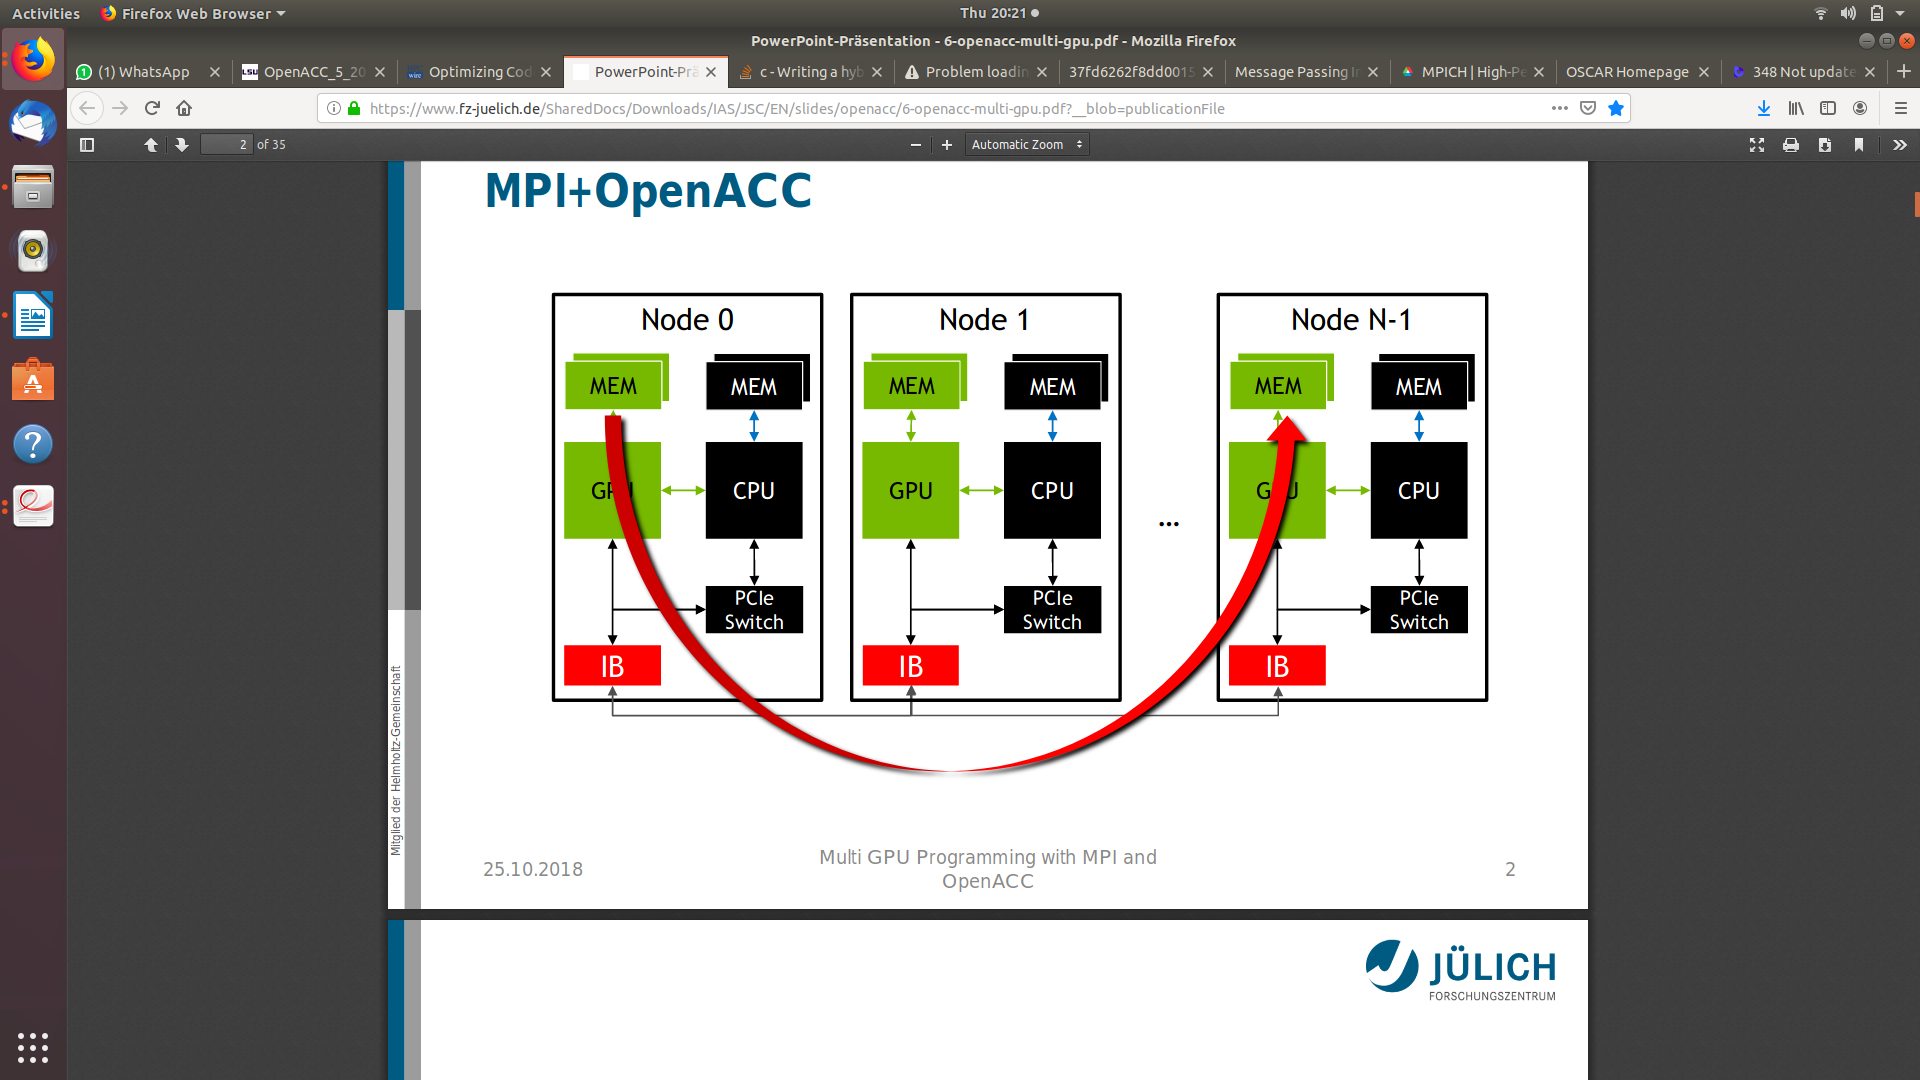
\includegraphics[width=14.631cm,height=7.689cm]{csn221Report-img001.png}
\end{center}

\bigskip

\subsection[]{}
\subsection{}
\subsection{}
\subsection{}
\subsection{}
\subsection{}
\subsection{}
\subsection{Why Linux}
We choose Linux as an operating system because Linux is well known for being an easy-to-use commodity, reliability and
fully free for all. No other Operating System allows for this level of versatility.

\subsubsection[why Fedora]{\bfseries why Fedora}
We initially planned on using OSCAR (Open Source Cluster Application Resourses) , which provided better support for
Fedora (RedHat OS)


\bigskip

\subsection[MPICH]{MPICH}
\textcolor{black}{MPICH is a high performance and widely portable implementation of the
}\textstyleStrongEmphasis{\textmd{\textcolor{black}{Message Passing Interface (MPI)}}}\textcolor{black}{ standard.}

{\color{black}
MPICH and its derivatives form the most widely used implementations of MPI in the world. They are used exclusively on
nine of the top 10 supercomputers (June 2016 ranking), including the world's fastest supercomputer: Taihu Light.}

\subsubsection[alternatives explored]{\rmfamily\bfseries alternatives explored}
We initially planned on using OSCAR (Open Source Cluster Application Resourses) , but faced numerous difficulties due to
old and \href{https://www.powerthesaurus.org/out-of-date/synonyms}{\textcolor{black}{out-of-date}} documentation . We
resorted to mpich due to beginner friendly guides. 


\bigskip

\subsection[OpenACC]{\textmd{OpenACC}}
\textcolor{black}{OpenACC is an open~specification for compiler directives for parallel programming. By using OpenACC,
developers~can rapidly accelerate existing C, C++, and Fortran applications using~high-level directives that help
retain application portability across processor architectures.}

{\color{black}
We already had a hands-on-experience of using OpenACC due to a workshop conducted by NVIDIA with the efforts of our
instructor .}

\section[]{}
\section[IMPLEMENTATION]{\textmd{\textcolor{black}{IMPLEMENTATION}}}
\subsection[Installing Fedora30]{\textmd{Installing Fedora30}}
\paragraph[Download Fedora 30 Workstation ISO File]{\color{black} Download Fedora 30 Workstation ISO File}
\textbf{\ \ }Once the ISO file is downloaded, then burn it either in USB drive or DVD and \ \ \ \ make it bootable.

\paragraph[Boot Your Target System with Bootable media (USB Drive or DVD)]{\color{black} Boot Your Target System with
Bootable media (USB Drive or DVD)}
\textcolor{black}{\ \ Reboot the target machine ,.Set the boot medium as USB or DVD from Bios \ \ \ \ settings so system
boots up with bootable media.}

\paragraph[Choose Start Fedora{}-Workstation{}-30 Live]{\color{black} Choose Start Fedora-Workstation-30 Live}
\textcolor{black}{\ \ When the system boots up with bootable media then we will get the following \ \ \ \ screen, to
begin with installation on your system's hard disk, choose ``}\textstyleStrongEmphasis{\textmd{\textcolor{black}{Start
\ \ \ \ Fedora-Workstation-30 Live}}}\textcolor{black}{{}``}

\paragraph[Select Install to Hard Drive Option]{\color{black} Select Install to Hard Drive Option}
\paragraph[Choose Installation destination and partition Scheme]{\color{black} Choose Installation destination and
partition Scheme}
\textcolor{black}{\ \ In the next screen we will see the local available hard disk, select the disk that \ \ \ \ that
contains the space freed earlier and then choose how you want to create \ \ \ \ partitions on it from storage
configuration tab.}

\ \ \ \ If you choose ``\textstyleStrongEmphasis{Automatic}{}'' partition scheme, then installer will create the
\ \ \ \ \ \ necessary partition for your system automatically but if you want to create your \ \ \ \ own customize
partition scheme then choose ``\textstyleStrongEmphasis{Custom}{}'' option.

\ \ \ \ After creating the suitable partition move to the next window, click on Done


\bigskip


\bigskip

\subsection[Configuring Mpich]{\textmd{Configuring Mpich}}
\#This unzips the tar file

\ \ \textit{tar -xzf mpich-3.3.1.tar.gz}

\ \ \#This enters the folder created on unzipping the tar file

\ \ \textit{cd \ mpich-3.3.1}

\ \ \#This will configure the prerequisites for cluster formation

\ \ .\textit{/configure -{}-disable-fortran}

\ \ \textit{make}

{\itshape
\ \ sudo make install}

\ \ \#If configuration is successful this command will give the version

\ \ \textit{mpiexec --version}


\bigskip

\subsection[Configuring Master Node]{\textmd{Configuring Master Node}}
\ \ \#Add the client computer's IP Addresses to /etc/hosts

\ \ \ \ \textit{cat /etc/hosts;}

\ \ \#This will create a new user named mpiuser 

\ \ \ \ \textit{sudo adduser mpiuser;}

\ \ \#This will let you set password for mpiuser

\ \ \ \ \textit{sudo passwd mpiuser;}

\ \ \#Setting up SSH


\bigskip


\bigskip

\ \ \#install ssh

\ \ \ \ \textit{sudo dnf install -y openssh-server;}

\ \ \#start ssh service on device

\ \ \ \ \textit{sudo systemctl start sshd.service;}

{\itshape
\ \ \ \ sudo systemctl enable sshd.service;}

\ \ \#login to the created user 'mpiuser'

\ \ \ \ \textit{su - mpiuser}

\ \ \#Generate SSH keys and copy them to the machines' list of authorized\_keys

\ \ \ \ \textit{ssh-keygen -t rsa}

{\itshape
\ \ \ \ ssh mpiuser@client mkdir -p .ssh}

{\itshape
\ \ \ \ cat .ssh/id\_rsa.pub {\textbar} ssh mpiuser@client 'cat {\textgreater}{\textgreater} .ssh/authorized\_keys'}

{\itshape
\ \ \ \ ssh mpiuser@client 'chmod 700 .ssh'}

{\itshape
\ \ \ \ chmod 640 .ssh/authorized\_keys}

\ \ \#This will create a folder in \$HOME for mpiuser named cloud that is shared in cluster

\ \ \ \ \textit{mkdir cloud}

{\itshape
\ \ \ \ exit}

\ \ \#Install NFS service 

\ \ \ \ \textit{sudo dnf -y install nfs-utils}

\ \ \#add the n=given folder to /etc/exports

\ \ \ \ \textit{echo {\textquotedbl}ADD /home/mpiuser/cloud *(rw,sync,no\_root\_squash,no\_subtree\_check) \ \ \ \ to
/etc/exports{\textquotedbl}}

\ \ \#This will open the /etc/exports folder in vi editor

\ \ \ \ \textit{sudo vi /etc/exports}

\ \ \#This should be run everytime ther is a change in /etc/exports

\ \ \ \ \textit{exportfs -a}

\ \ \#this will start the nfs service

\ \ \ \ \textit{sudo systemctl start rpcbind nfs-server}

{\itshape
\ \ \ \ sudo systemctl enable rpcbind nfs-server}


\bigskip

\ \ \textit{echo {\textquotedbl}ssh and nfs have been setUp{\textbackslash}n add all cluster IPs to
/etc/hosts{\textquotedbl}}

\subsection[Configuring Client Node]{\textmd{Configuring Client Node}}
\#Add the client computer's IP Addresses to /etc/hosts

{\itshape
\ \ cat /etc/hosts;}

\textit{\ \ }\#This will create a new user named mpiuser 

{\itshape
\ \ sudo adduser mpiuser;}

\#This will let you set password for mpiuser

{\itshape
\ \ sudo passwd mpiuser;}


\bigskip


\bigskip


\bigskip

\#Setting up SSH

\#install ssh

{\itshape
\ \ sudo dnf install -y openssh-server;}

\#start ssh service on device

\ \ sudo systemctl start sshd.service;

\ \ sudo systemctl enable sshd.service;

\#login to the created user 'mpiuser'

\textit{\ \ su - mpiusera}

\textit{\ \ }\#Generate SSH keys and copy them to the machines' list of authorized\_keys

{\itshape
\ \ ssh-keygen -t rsa}

{\itshape
\ \ \ \ ssh mpiuser@master mkdir -p .ssh}

{\itshape
\ \ cat .ssh/id\_rsa.pub {\textbar} ssh mpiuser@master 'cat {\textgreater}{\textgreater} .ssh/authorized\_keys'}

{\itshape
\ \ ssh mpiuser@master 'chmod 700 .ssh'}

{\itshape
\ \ chmod 640 .ssh/authorized\_keys}

\#This will create a folder in \$HOME for mpiuser named cloud that is shared in cluster

{\itshape
\ \ mkdir cloud}

{\itshape
\ \ exit}

\textit{\ \ }\#Install NFS service

{\itshape
\ \ sudo dnf -y install nfs-utils}

\#mount the shared directory

{\itshape
\ \ sudo mount -t nfs master:/home/mpiuser/cloud /home/mpiuser/cloud}

\#to check the mounted directories

{\itshape
\ \ df -h}

\#Create a systems table in /etc/fstab

{\itshape
\ \ echo {\textquotedbl}Add master:/home/mpiuser/cloud /home/mpiuser/cloud nfs \ to /etc/fstab{\textquotedbl}}

{\itshape
\ \ sudo vi /etc/fstab}

\paragraph{}
\ \ \textbf{\textit{Problems encountered: }}Firewall hinders in the communication established by MPICH,

\ \ thus throwing NFS (Network File System) errors , thus firewall had to be disabled


\bigskip


\bigskip

\subsection[Understanding and implementing Jacobi Method]{\textmd{Understanding and implementing Jacobi Method}}
Let 



\begin{center}
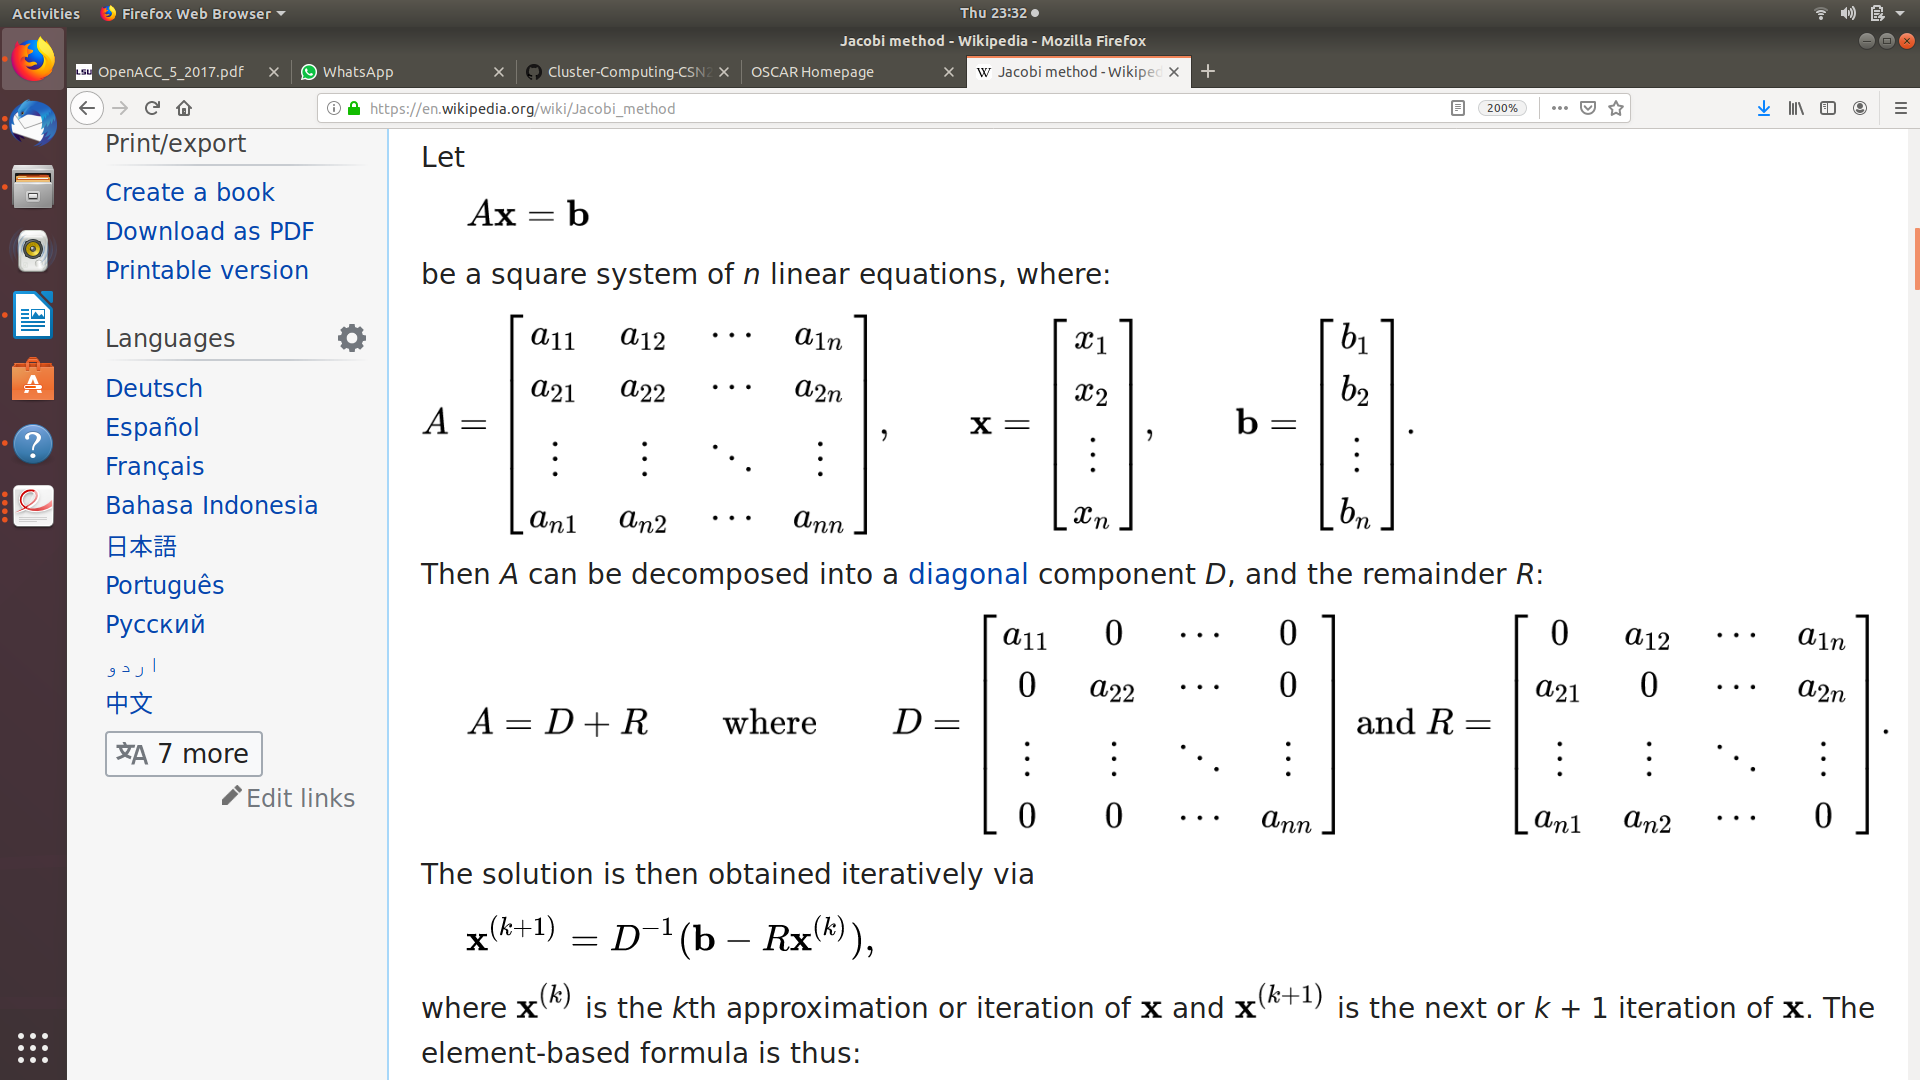
\includegraphics[width=8.844cm,height=1.914cm]{csn221Report-img002.png}
\end{center}

\bigskip

be a square system of \textit{n} linear equations, where:


\bigskip

\ 

\begin{center}
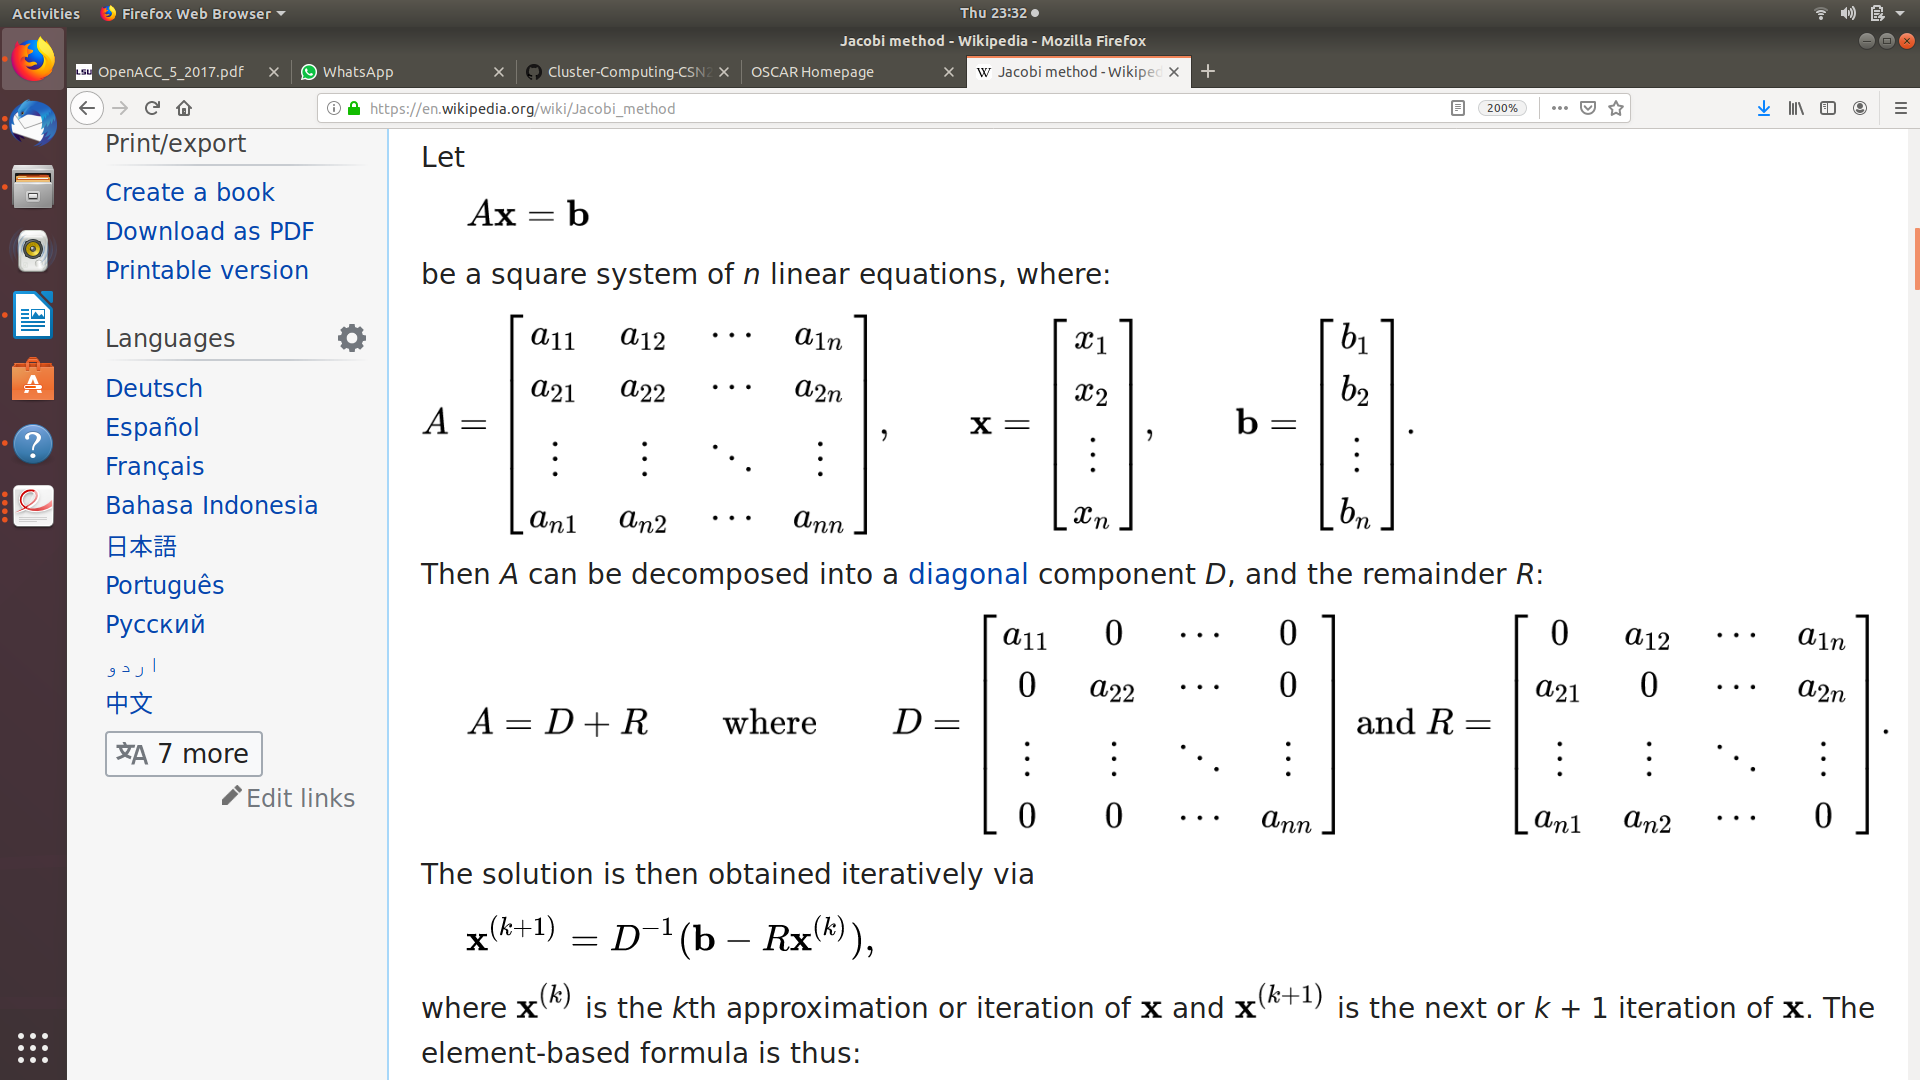
\includegraphics[width=16.905cm,height=3.895cm]{csn221Report-img002.png}
\end{center}
 
\includegraphics[width=0.041cm,height=0.041cm]{csn221Report-img003.png} 


\bigskip


\bigskip


\bigskip


\bigskip

Then \textit{A} can be decomposed into a
\href{https://en.wikipedia.org/wiki/Diagonal_matrix}{\textcolor{black}{diagonal}} component \textit{D}, and the
remainder \textit{R}: 



\begin{center}
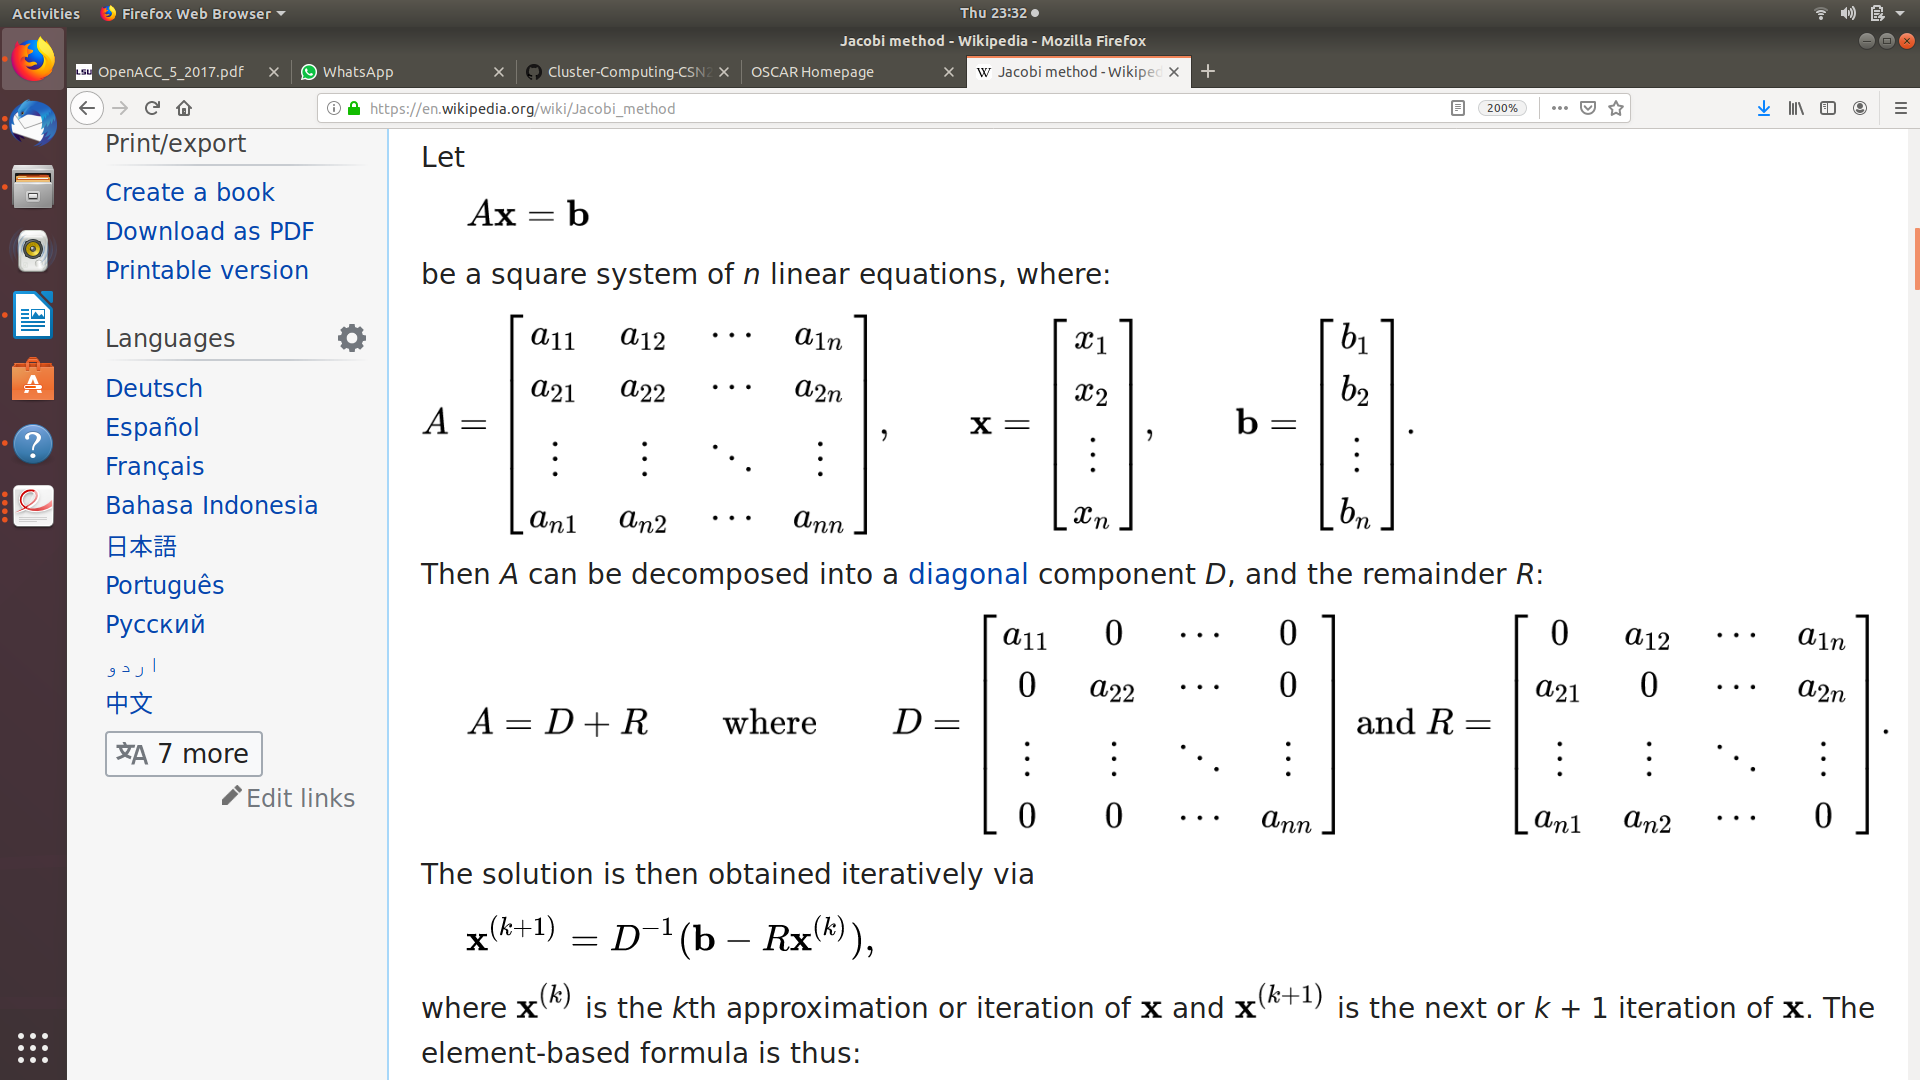
\includegraphics[width=18.376cm,height=2.969cm]{csn221Report-img002.png}
\end{center}
The solution is then obtained iteratively via 



\begin{center}
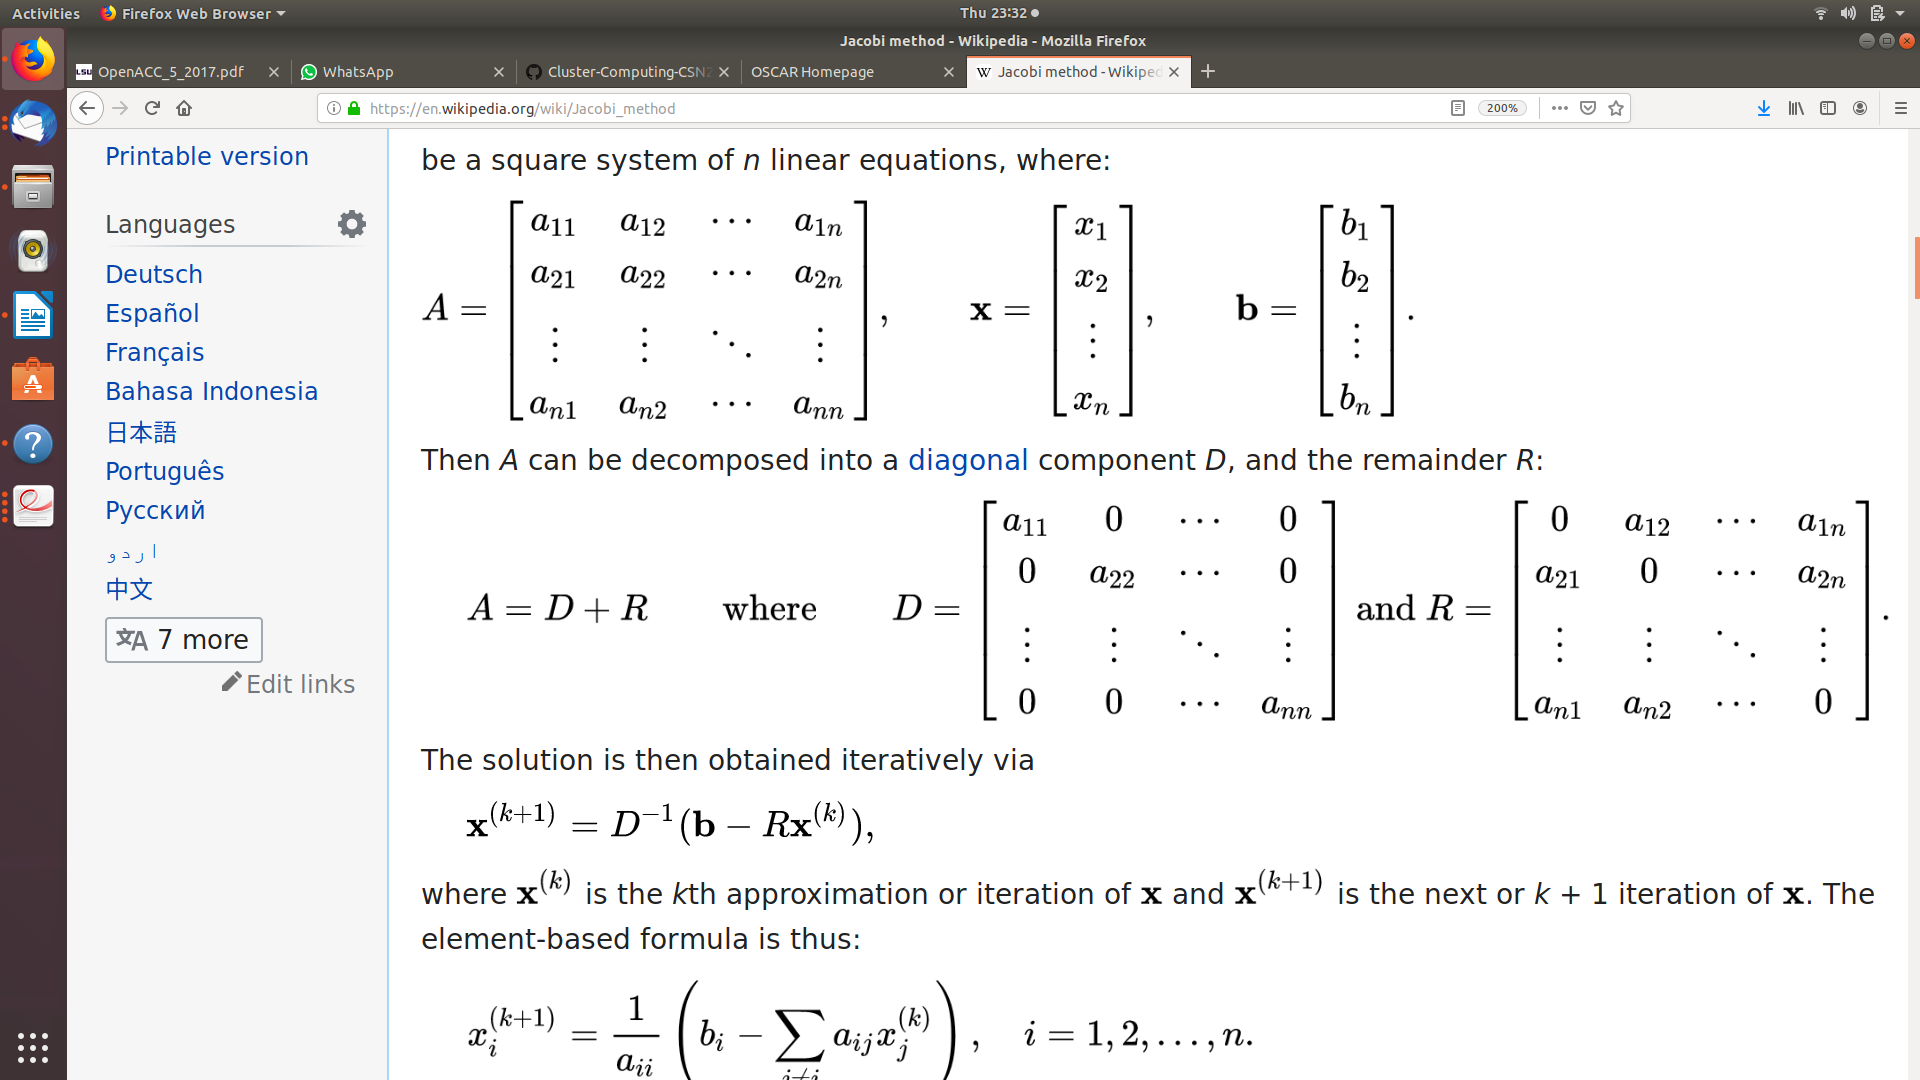
\includegraphics[width=9.409cm,height=1.358cm]{csn221Report-img004.png}
\end{center}
 
\includegraphics[width=0.041cm,height=0.041cm]{csn221Report-img003.png} 


\bigskip

where  
\includegraphics[width=0.041cm,height=0.041cm]{csn221Report-img003.png} \ is the \textit{k}th approximation or
iteration of  
\includegraphics[width=0.041cm,height=0.041cm]{csn221Report-img003.png} \ and 

\includegraphics[width=0.041cm,height=0.041cm]{csn221Report-img003.png} \ is the next or \textit{k} + 1 iteration of 

\includegraphics[width=0.041cm,height=0.041cm]{csn221Report-img003.png} . The element-based formula is thus: 



\begin{center}
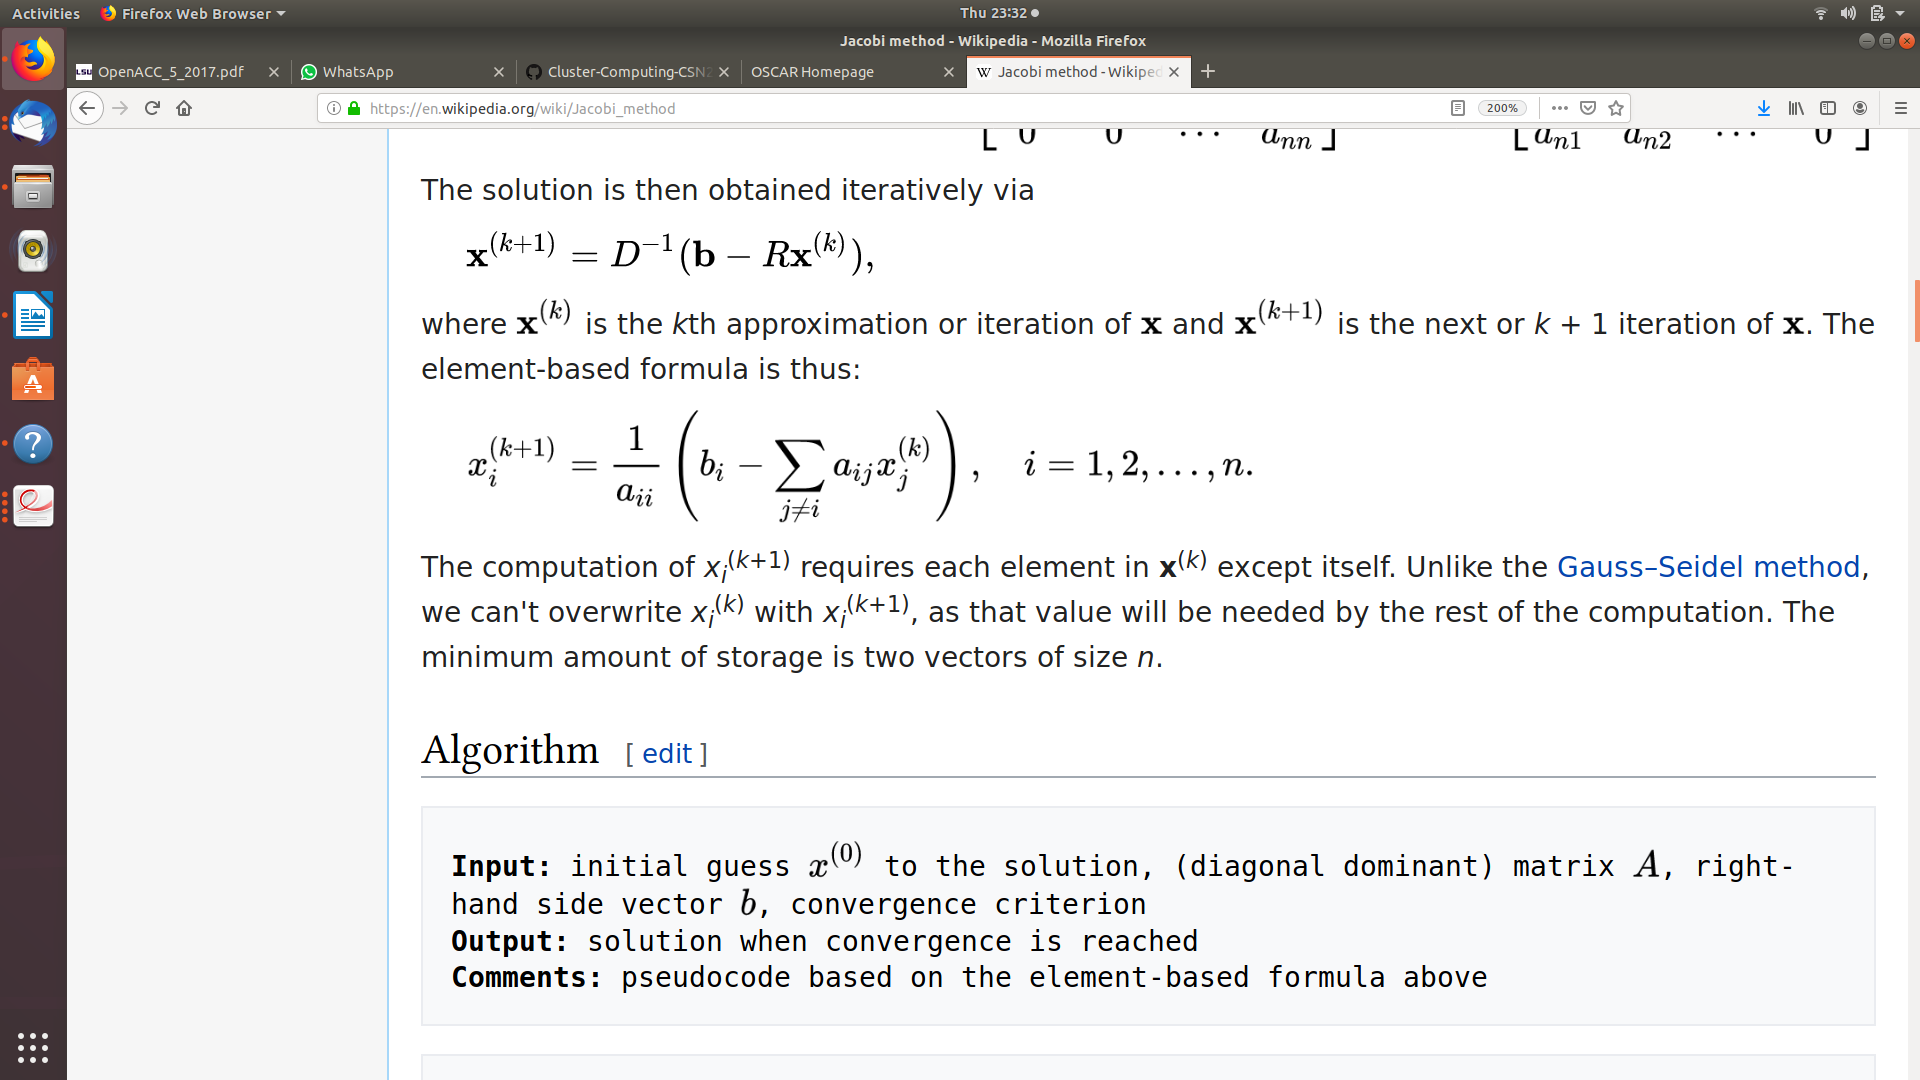
\includegraphics[width=14.658cm,height=2.334cm]{csn221Report-img005.png}
\end{center}
 
\includegraphics[width=0.041cm,height=0.041cm]{csn221Report-img003.png} 


\bigskip

The computation of
\textit{x}\textit{\textsubscript{i}}\textsuperscript{(}\textit{\textsuperscript{k}}\textsuperscript{+1)} requires each
element in \textbf{x}\textsuperscript{(}\textit{\textsuperscript{k}}\textsuperscript{)} except itself. Unlike the
\href{https://en.wikipedia.org/wiki/Gauss?Seidel_method}{Gauss--Seidel method}, we can't overwrite
\textit{x}\textit{\textsubscript{i}}\textsuperscript{(}\textit{\textsuperscript{k}}\textsuperscript{)} with
\textit{x}\textit{\textsubscript{i}}\textsuperscript{(}\textit{\textsuperscript{k}}\textsuperscript{+1)}, as that value
will be needed by the rest of the computation. The minimum amount of storage is two vectors of size \textit{n}


\bigskip

\subsection[Identifying loops to be parallelized]{\rmfamily Identifying loops to be parallelized}
Identify section of a code consuming the significant percentage of time (hot spots). We used gprof (profiling tool ) to
analyze the execution time.

\subsection[Using kernal construct to parallelize ]{\rmfamily Using kernal construct to parallelize }
The kernels construct expresses that a region may contain parallelism and the compiler determines what can safely be
parallelized.

\ \ \ \ \ \ \ \ \textbf{\#pragma acc kernels}

\ \ \ \ \ \ \ \ for (int j = jstart; j {\textless} jend; j++)

\ \ \ \ \ \ \ \ \{

\ \ \ \ \ \ \ \ \ \ \ \ for( int i = 1; i {\textless} M-1; i++ )

\ \ \ \ \ \ \ \ \ \ \ \ \{

\ \ \ \ \ \ \ \ \ \ \ \ \ \ \ \ Anew[j][i] = 0.25f * ( A[j][i+1] + A[j][i-1]

\ \ \ \ \ \ \ \ \ \ \ \ \ \ \ \ \ \ \ \ \ \ \ \ \ \ \ \ \ \ \ \ \ \ \ \ \ + A[j-1][i] + A[j+1][i]);

\ \ \ \ \ \ \ \ \ \ \ \ \ \ \ \ error = fmaxf( error, fabsf(Anew[j][i]-A[j][i]));

\ \ \ \ \ \ \ \ \ \ \ \ \}

\ \ \ \ \ \ \ \ \}

\ \ \ \ \ \ \ \ \textbf{\#pragma acc kernels}

\ \ \ \ \ \ \ \ for( int i = 1; i {\textless} M-1; i++ )

\ \ \ \ \ \ \ \ \{

\ \ \ \ \ \ \ \ \ \ \ \ \ \ \ \ A[jstart][i] = Anew[jstart][i];

\ \ \ \ \ \ \ \ \ \ \ \ \ \ \ \ A[jend-1][i] = Anew[jend-1][i];

\ \ \ \ \ \ \ \ \}


\bigskip

\ \ \ \ \ \ \ \textbf{\ \#pragma acc kernels async}

\ \ \ \ \ \ \ \ for (int j = (jstart+1); j {\textless} (jend-1); j++)

\ \ \ \ \ \ \ \ \{

\ \ \ \ \ \ \ \ \ \ \ \ for( int i = 1; i {\textless} M-1; i++ )

\ \ \ \ \ \ \ \ \ \ \ \ \{

\ \ \ \ \ \ \ \ \ \ \ \ \ \ \ \ A[j][i] = Anew[j][i];

\ \ \ \ \ \ \ \ \ \ \ \ \}

\ \ \ \ \ \ \ \ \}

\subsection[Distributing processes using mpich]{\rmfamily Distributing processes using mpich}
\subsection[Building the project]{\rmfamily Building the project}
all: run

laplace2d: laplace2d.c common.h laplace2d\_serial.h Makefile

\ \ mpicc -Ofast -pg laplace2d.solution.c -lm -o laplace2d 

clean:

\ \ rm -f laplace2d

run: laplace2d

\ \ mpirun -np 9 -{}-hosts rg,client,client2 ./laplace2d

profile: laplace2d

\ \ mpirun -np 2 nvprof -o laplace2d.\%q\{OMPI\_COMM\_WORLD\_RANK\}.nvvp ./laplace2d


\bigskip


\bigskip

\section[]{}

\bigskip


\bigskip


\bigskip


\bigskip


\bigskip


\bigskip


\bigskip


\bigskip


\bigskip


\bigskip


\bigskip


\bigskip


\bigskip


\bigskip

\section[]{}

\bigskip

\section[TESTING]{\textcolor{black}{TESTING}}

\bigskip



\begin{center}
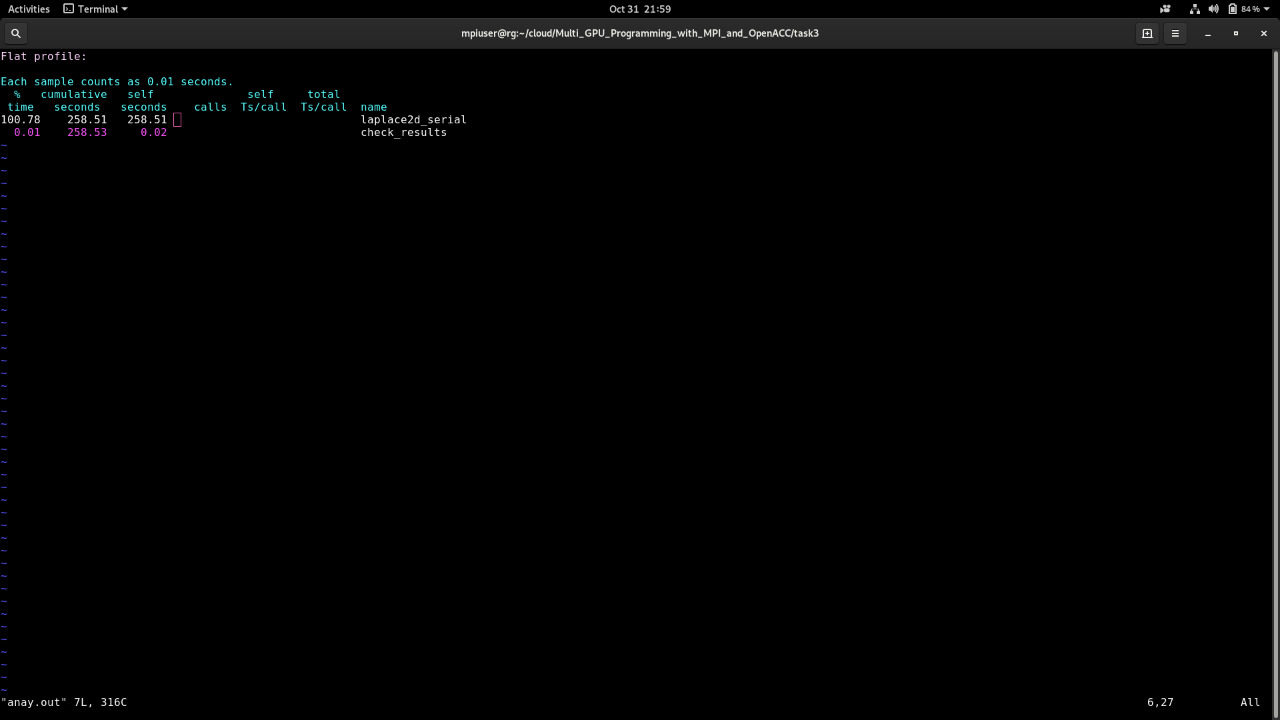
\includegraphics[width=19.812cm,height=6.911cm]{csn221Report-img006.jpg}
\end{center}
\begin{center}
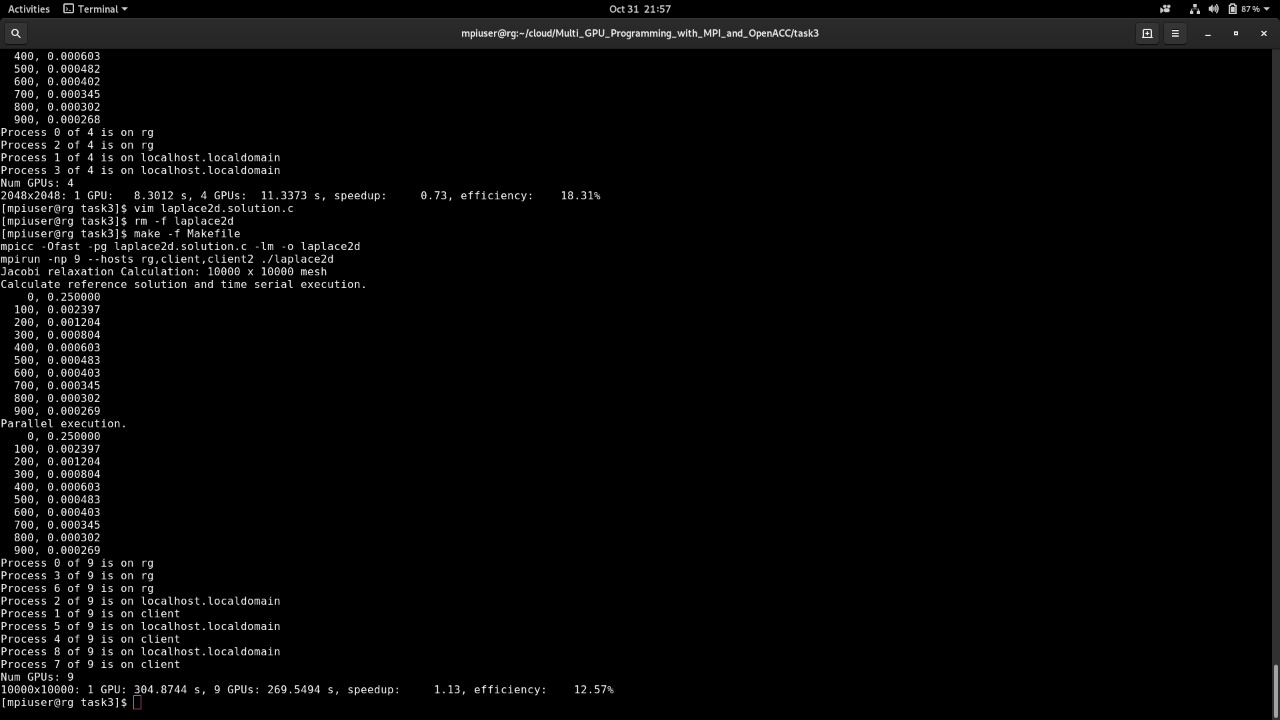
\includegraphics[width=18.867cm,height=9.065cm]{csn221Report-img007.jpg}
\end{center}

\bigskip

\section[]{\color{black} }

\bigskip


\bigskip


\bigskip

\section[]{\color{black} }
\section[]{\color{black} }
\section[]{\color{black} }
\section[]{\color{black} }
\section[RESULT AND CONCLUSION]{\color{black} \textstyleFootnoteSymbol{RESULT AND CONCLUSION}}
{\color{black}
\textstyleFootnoteSymbol{We noted a speedup of 1.13 . Although it can be noted that the efficiency is low.}}

\textstyleFootnoteSymbol{\textcolor{black}{This is a drawback of
Be}\textcolor{black}{o}\textcolor{black}{w}\textcolor{black}{u}\textcolor{black}{lf }\textcolor{black}{like cluster
,}\textcolor{black}{t}\textcolor{black}{hey add complexity in terms of both designing the different heterogeneous
elements and the additional programming effort to decide when and how to make use of the varying resources . Symmetric
MPI applications will assign identical workloads to all participants in the application, which can cause load
imbalance, as the execution time might be shorter on some devices due to their higher computational performance. MPI
synchronization events will show this load imbalance because high-performance devices will be idle while they wait for
slower devices to catch up. ITAC can visualize MPI communication and allows spotting those situation(s), where some MPI
ranks must wait a significant amount of time for the synchronization with slower components of the heterogeneous
cluster.}\textcolor{black}{There is also additional communication time which negatively effects the efficiency.}}


\bigskip


\bigskip


\bigskip


\bigskip


\bigskip


\bigskip


\bigskip


\bigskip


\bigskip


\bigskip


\bigskip


\bigskip


\bigskip


\bigskip


\bigskip


\bigskip


\bigskip


\bigskip


\bigskip


\bigskip

{\centering
\textstyleFootnoteSymbol{\textcolor{black}{REFERENCES}}
\par}

\textstyleFootnoteSymbol{\textcolor{black}{[1] The Open Cluster Group ,
}}\href{http://www.OpenClusterGroup.org/}{\textstyleFootnoteSymbol{http://www.OpenClusterGroup.org}}

\textstyleFootnoteSymbol{\textcolor{black}{[2] MPICH, \ \ }}\url{http://www-unix.mcs.anl.gov/mpi/mpich}

\textstyleFootnoteSymbol{\textcolor{black}{[3] OpenMP for Next Generation Heterogeneous Clusters,
\ \ \ \ }}\url{https://www.usenix.org/conference/}\textstyleFootnoteSymbol{\textcolor{black}{ \ \ \ \ \ \ \ }}

\textstyleFootnoteSymbol{\textcolor{black}{\ \ \ \ \ \ hotpar-10/openmp-next-generation-heterogeneous-clusters}}

\textstyleFootnoteSymbol{\textcolor{black}{[4] }\textcolor{black}{Analysis and Implementation of Cluster Computing Using
Linux}}

\textstyleFootnoteSymbol{\textcolor{black}{\ \ \ \ \ Operating System , IOSR Journal of Computer Engineering (IOSRJCE)}}

\textstyleFootnoteSymbol{\textcolor{black}{\ \ \ \ \ ISSN: 2278-0661 Volume 2, Issue 3 (July-Aug. 2012), PP 06-11}}

\textstyleFootnoteSymbol{\textcolor{black}{[5] The implementations of multi-level heterogeneous parallel computation
with MPI and }}

\textstyleFootnoteSymbol{\textcolor{black}{\ \ \ \ \ \ OpenACC : https://doi.org/10.1190/IGC2017-061}}
\end{document}
